% !Tex program = pdflatex
% 第 14 章: 光辐射的调制
\ifx\allfiles\undefined
\documentclass{note}
\begin{document}
\fi
\setcounter{chapter}{13}
\chapter{光辐射的调制}
\begin{exe}
    推导九个椭圆的方程式, 这些椭圆是由如图 14.3c 所示的光场矢量 (作为位相延迟 $\Gamma$ 的函数) 描绘出来的.
\end{exe}
\begin{pf}
    $x'$ 和 $y'$ 方向的光场矢量分别为
    \begin{align}
        \label{14.1-1}
        E_{x'}=A\cos\left[\omega t-\left(\frac{\omega}{c}\right)\left(n_o-\frac{n_o^3}{2}r_{63}E_z\right)z\right],\\
        \label{14.1-2}
        E_{y'}=A\cos\left[\omega t-\left(\frac{\omega}{c}\right)\left(n_o+\frac{n_o^3}{2}r_{63}E_z\right)z\right].
    \end{align}
    这两个矢量的相位差为
    \begin{align}
        \Gamma=\frac{\omega n_o^3r_{63}}{c}E_zz.
    \end{align}
    将这两个矢量分别重写为
    \begin{align}
        E_{x'}=&A\cos(\omega t-kz+\Gamma/2)=A[\cos(\omega t-kz)\cos(\Gamma/2)-\sin(\omega t-kz)\sin(\Gamma/2)],\\
        E_{y'}=&A\sin(\omega t-kz-\Gamma/2)=A[\cos(\omega t-kz)\cos(\Gamma/2)+\sin(\omega t-kz)\sin(\Gamma/2)],
    \end{align}
    其中 $k=\frac{n_o\omega}{c}$,
    从而
    \begin{align}
        \sin(\omega t-kz)=&\frac{E_{y'}-E_{x'}}{2A\sin(\Gamma/2)},\\
        \cos(\omega t-kz)=&\frac{E_{y'}+E_{x'}}{2A\cos(\Gamma/2)}.
    \end{align}
    利用
    \begin{align}
        \sin^2(\omega t-kz)+\cos^2(\omega t-kz)=1
    \end{align}
    得
    \begin{align}
        E_{x'}^2+E_{y'}^2-2E_{x'}E_{y'}\cos\Gamma=A^2\sin^2\Gamma.
    \end{align}
\end{pf}

\begin{exe}
    讨论式 (14.5-1) 中与场无关的延迟 $(\omega l/c)(n_o-n_e)$ 对振幅调制器 (如图 14.4 所示) 的影响.
\end{exe}
\begin{sol}
    横向调制时 $z$ 方向和 $x'$ 方向的相位延迟为式 (14.5-1):
    \begin{align}
        \Gamma=\phi_z-\phi_x'=\frac{\omega l}{c}\left[(n_o-n_e)-\frac{n_o^3}{2}r_{63}\left(\frac{V}{d}\right)\right].
    \end{align}
    设入射光的 $x'$ 方向和 $z$ 方向的电场矢量分别为
    \begin{align}
        E_x'(0)=&A,\\
        E_z(0)=&A,
    \end{align}
    则入射光强度
    \begin{align}
        I_i\propto\abs{E_x'(0)}^2+\abs{E_z(0)}^2=2A^2,
    \end{align}
    从电光晶体出射的光的 $x'$ 方向和 $z$ 方向电场矢量可分别写为
    \begin{align}
        E_x'(l)=&A,\\
        E_z(l)=&Ae^{-i\Gamma},
    \end{align}
    从检偏振器出射的光的电场矢量为
    \begin{align}
        E_o=\frac{1}{\sqrt{2}}[E_x'(l)-E_z(l)]=\frac{A}{\sqrt{2}}(e^{-i\Gamma}-1)
    \end{align}
    从检偏振器出射的光强
    \begin{align}
        I_o\propto\abs{E_o}^2=\frac{A^2}{2}(e^{-i\Gamma}-1)(e^{i\Gamma}-1)=2A^2\sin^2\frac{\Gamma}{2}.
    \end{align}
    出射光和入射光强度之比为
    \begin{align}
        \frac{I_o}{I_i}=\sin^2\frac{\Gamma}{2}.
    \end{align}
    由于式 (14.5-1) 中与场无关的延迟 $(\omega l/c)(n_o-n_e)$ 依赖温度, 故振幅调制器的透射率可能随环境温度发生漂移.
\end{sol}

\begin{exe}
    用 $\sin(a\sin x)$ 的贝塞尔函数展开式并根据调制频率 $\omega_m$ 的谐振函数来表示式 (14.3-7). 划出出射强度的三次谐波 ($3\omega_m$) 与基波的比值随 $\Gamma_m$ 的变化曲线. 若比值不超过 $10^{-2}$, 问最大允许的 $\Gamma_m$ 是多少?\\
    答案: $\Gamma_m<0.5$.
\end{exe}
\begin{sol}
    由式 (14.3-7), 交变电压调制下出射光强与入射光强之比为
    \begin{align}
        \frac{I_o}{I_i}=\frac{1}{2}[1+\sin(\Gamma_m\sin\omega_mt)].
    \end{align}
    利用
    \begin{align}
        \sin(z\sin\phi)=2\sum_{n=0}^{\infty}J_{2n+1}(z)\sin[(2n+1)\phi],
    \end{align}
    可将上式展开为
    \begin{align}
        \frac{I_o}{I_i}=\frac{1}{2}+\sum_{n=0}^{\infty}J_{2n+1}(\Gamma_m)\sin[(2n+1)\omega_mt].
    \end{align}
    其中三次谐波 ($3\omega_m$) 与基波的比值随 $\Gamma_m$ 的变化曲线如图 \ref{14.3} 所示.
    \begin{figure}[H]
        \centering
        \subfigure{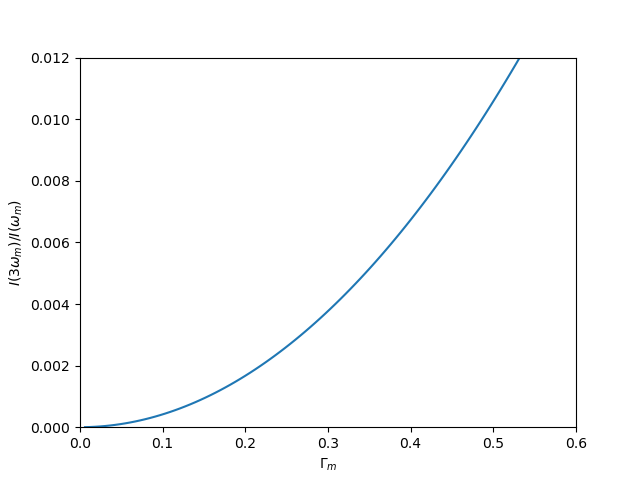
\includegraphics[width=.4\columnwidth]{Figures/14.3-1.png}}
        \subfigure{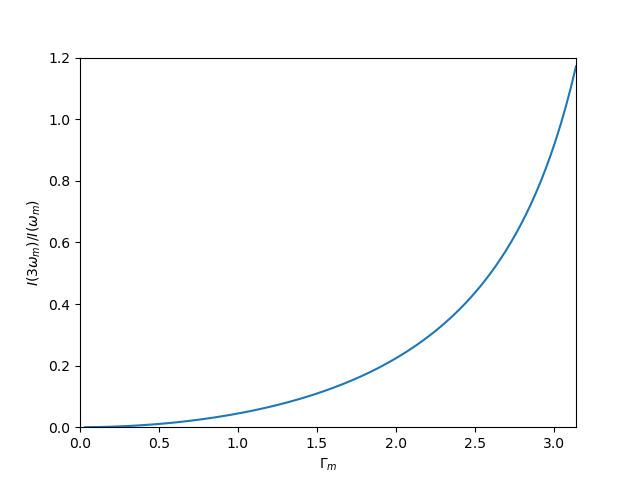
\includegraphics[width=.4\columnwidth]{Figures/14.3-2.png}}
        \caption{出射强度的三次谐波 $(3\omega_m)$ 与基波的比值随 $\Gamma_m$ 的变化曲线.}
        \label{14.3}
    \end{figure}
    由上图知, 若要求该比值不超过 $10^{-2}$, 则最大允许的 $\Gamma_m$ 为 $0.5$.
\end{sol}

\begin{exe}
    试证明, 如一位相调制光波入射在一平方律探测器上, 则输出中只有直流成分.
\end{exe}
\begin{pf}
    
\end{pf}

\begin{exe}
    利用参考文献 [8] 和 [9], 设计一个在频率 $\nu_m=10^9$ 赫时运转的部分负载 KDP 位相调制器并得到 $\delta=\pi/3$ 峰值位相偏移. 问调制功率是多少?
\end{exe}
\begin{sol}
    
\end{sol}

\begin{exe}
    推导型号如 14.5 节举例中所描述的横向 $\bar{4}3m$ 晶体光电调制器的调制功率的表达式 (类似式 (14.6-2)).
\end{exe}
\begin{pf}
    
\end{pf}

\begin{exe}
    \begin{itemize}
        \item[(a)] 试证明, 在如图 14.4 装置中光线与 $z$ 轴成 $\theta$($\ll$) 的角度传播, 它使双折射对位相延迟的影响为
        \[
            \Delta\Gamma_{\text{双折射}}=\frac{\omega l}{2c}n_0\left(\frac{n_0^2}{n_e^2}-1\right)\theta^2.
        \]
        相应的折射率变化为
        \[
            n_0-n_e(\theta)=\frac{n_0\theta^2}{2}\left(\frac{n_0^2}{n_e^2}-1\right).
        \]
        \item[(b)] 导出最大允许束散角的近似表达式, 在此束散角下 $\Delta\Gamma_{\text{双折射}}$ 并不妨碍调制器的运转.
    \end{itemize}
    答案:
    \[
        \theta<\left[\frac{\lambda}{4n_0l\left(\frac{n_0^2}{n_e^2}-1\right)}\right]^{1/2}.
    \]
\end{exe}
\begin{sol}
    \begin{itemize}
        \item[(a)] 
        \item[(b)] 
    \end{itemize}
\end{sol}

\begin{exe}
    查阅文献 (例如可阅读文献 [17] 和 [18]) 并阐述布拉格衍射和德拜-西尔斯 (Debye-Sears) 衍射之间的差别. 在什么条件下可观察到每种衍射?
\end{exe}
\begin{sol}
    
\end{sol}

\begin{exe}
    晶体中 $X$ 射线衍射的布拉格定律为
    \[
        2d\sin\theta=m\frac{\lambda}{n},\quad m=1,2,3
    \]
    式中 $n$ 为折射率, $d$ 为等价原子平面间的距离, $\theta$ 为入射角, 而 $\lambda$ 为衍射辐射在真空中的波长. 当 $2\lambda_s\sin\theta=\frac{\lambda}{n}$ 时光与声波作用而产生布拉格衍射 (参见图 14.15). 与 X 射线衍射结果相比较并取 $\lambda_s=d$, 则只有 $m=1$ 的情况是允许的. 解释其差别. 对于受声波散射的情况, 为什么不能得到对应于 $m=2,3,\cdots$ 的衍射角 $\theta$ 呢?\\
    提示: X 射线衍射发生在分立的原子平面上, 它可被理想化为无限薄的薄片, 而声波的扰动则是正弦曲线的.
\end{exe}
\begin{sol}
    
\end{sol}

\begin{exe}
    对 $\Delta k=\abs{\bm{k}_i-\bm{k}_s-\bm{k}_d}\neq 0$ 和小输入信号 $E_i(0)$ 的情况, 解耦合模方程 (14.9-8). 假设有共线相互作用, 则 $r_i=r_d=r_s=z$. 试证明入射功率转化为衍射光束的最大比率为
    \[
        \frac{\eta^2}{\eta^2+\left(\frac{\Delta k}{2}\right)^2}.
    \]
    可见, 可允许的失配量 $\Delta k$ 同 $\eta$ 有关. 你能对违反动量守恒作出直观的解释吗?
\end{exe}
\begin{pf}
    
\end{pf}

\begin{exe}
    从多普勒理论和式 (14.9-12) 推导出式 (14.9-11).
\end{exe}
\begin{pf}
    
\end{pf}
\ifx\allfiles\undefined
\end{document}
\fi